\documentclass[../Assignment-3-LPSMT.tex]{subfiles}
\graphicspath{{\subfix{../img/}}}

\begin{document}

\chapter{Wireframe e navigazione}

\section{Digressione Material Design}

Le interfacce grafiche dell'applicazione sono state realizzate seguendo il più possibile gli standard imposti da Material Design 3~\cite{matDes}.\\
In alcuni casi come nella ricerca dell'indice all'interno del \hyperref[sec:reader]{Reader} abbiamo preferito divergere delle linee guida di Material Design 3 per una UX migliore da parte dell'utente.

\section{Mock-up}

Test sono una prova

\subsection{Library \- Home page}\label{sec:home}

\begin{center}
   \includegraphics[scale=0.4]{library_home_page.png}
\end{center}

L'applicazione si avvierà nella schermata contenente la libreria del lettore.\\
La libreria presenterà le opere possedute dall'utente ognuna contrassegnata dal nome.\\
Cliccando sull'anteprima di uno dei fumetti verrà aperta la \hyperref[sec:comic_list]{Comic List}, mentre premendo sull'icona nell'angolo superiore sinistro verrà aperto un \hyperref[sec:hamburger]{Menù ad hamburger}.\\
Nell'angolo in basso a destra sarà presente un bottone per aggiungere una nuova opera le cui informazioni verranno recuperate dal database remoto che fa da supporto all'applicazione, le informazioni recuperate saranno titolo, immagine di anteprima, breve descrizione, $\dots$\\
La ricerca nel database verrà effettuata tramite il fragment \hyperref[sec:add_library]{Add Library}

\subsection{Comic List}\label{sec:comic_list}

\begin{center}
  \includegraphics[scale=0.4]{comic_list.png}
\end{center}

In questa schermata l'utente troverà la lista dei volumi/capitoli, di un'opera, che ha caricato all'interno dell'applicazione.\\
Con il tasto ``+'' posizionato nell'angolo inferiore destro potrà aggiungere un nuovo capitolo/volume associato all'opera, mentre tenendo premuto sul nome di un elemento della lista potrà aggiornarne gli attributi tramite il form presente in \hyperref[sec:update_comic]{Update Comic}.\\
Infine premendo su un volume/capitolo si verrà portati al \hyperref[sec:reader]{Reader}.

\subsection{File Manager}

\begin{center}
  \includegraphics[scale=0.4]{file_manager.png}
\end{center}

L'applicazione dovrà interfacciarsi con il file manager per poter permettere all'utente di selezionare i file \emph{.cbz} da caricare.\\
Una volta selezionato il file si verrà portati nel fragment \hyperref[sec:add_chapter]{Add chapter}.

\subsection{Add Chapter}\label{sec:add_chapter}

\begin{center}
  \includegraphics[scale=0.4]{add_chapter.png}
\end{center}

Tramite un breve form l'utente potrà modificare il nome del file e indicare che capitolo sta inserendo.\\
Il capitolo indicato dall'utente non andrà in alcun modo a modificare i contenuti della \hyperref[sec:reading_list]{Reading List} ma servirà solo a mantenere una numerazione all'interno della vista \hyperref[sec:comic_list]{Comic List}.

\subsection{Update Comic}\label{sec:update_comic}

\begin{center}
  \includegraphics[scale=0.4]{update_library.png}
\end{center}

Tramite un dialog simile a \hyperref[sec:add_chapter]{Add Chapter} l'utente potrà andare a modificare i dati con cui è stato salvato il capitolo/volume dell'opera selezionata.

\subsection{Add Library}\label{sec:add_library}

\begin{center}
  \includegraphics[scale=0.4]{add_library.png}
\end{center}

Tramite una casella di testo l'utente potrà interrogare il database remoto così d'aggiungere in locale una nuova opera con le relative informazioni.

\subsection{Reader}\label{sec:reader}

\begin{center}
   \includegraphics[scale=0.4]{reader.png}
\end{center}

La schermata del Reader conterrà una barra di navigazione nel lato inferiore dello schermo.\\
La barra di navigazione avrà dei comandi basici per muoversi all'interno del file, un bottone per andare alla pagina precedente, uno per andare a quella successiva e uno per ricercare la pagina con un determinato numero.\\
Il numero con cui si effettuerà la ricerca sarà assoluto e.g.\ la copertina sarà la pagina numero 1.\\
Nella parte superiore dello schermo sarà presente una freccia per poter tornare alla \ignore{\hyperref[sec:home]{Library \- Home page}} schermata dell'opera e interrompere la lettura.

\subsection{Search dialog}

\begin{center}
   \includegraphics[scale=0.4]{search_dialog.png}
\end{center}

Una volta premuto sull'icona della ricerca verrà aperto un dialog dove verrà chiesto all'utente di inserire l'indice della pagina alla quale si vuole andare.\\
Il formato di file scelto, ovvero \emph{.cbz}, non contiene metadati per l'enumerazione, quindi la numerazione inizia con la prima schermata che avrà indice 1.\\
Questa potrebbe essere una debolezza ma ogni altro lettore di \emph{.cbz} contiene questa imperfezione.

\subsection{Menù ad hamburger}\label{sec:hamburger}

\begin{center}
   \includegraphics[scale=0.4]{hamburger.png}
\end{center}

Il Menù ad hamburger conterrà lo user name se l'utente è autenticato, altrimenti lascerà uno spazio vuoto.\\
Il resto del menù conterrà una lista con le seguenti voci:
\begin{itemize}
   \item \textbf{Reading list} che porterà l'utente alla propria lista delle letture.
   \item \textbf{FTP server} permetterà all'utente di configurare il proprio server FTP dal quale dopo scaricare materiale.
   \item \textbf{Log in/out} sarà una stringa adattiva, se l'utente non è autenticato presenterà la scritta ``Log In'' altrimenti la scritta ``Log Out''.
  \item \textbf{Sign Up} permetterà all'utente di registrare un nuovo profilo, sarà presente solo se l'utente deve ancora effettuare l'accesso.
  \item \textbf{Library} creerà una shortcut per poter tornare alla \hyperref[sec:home]{Library \- Home page}.
\end{itemize}

\subsection{Reading list}\label{sec:reading_list}

\begin{center}
   \includegraphics[scale=0.4]{reading_list.png}
\end{center}

La reading list conterrà una lista delle letture che sono state inserite dall'utente.\\
Queste letture saranno divise in più categorie:
\begin{itemize}
   \item \textbf{Reading} conterrà le opere ch l'utente sta leggendo.\\
   In questa lista affiancato al nome delle opere ci sarà un indicatore del capitolo al quale si è arrivati.
   \item \textbf{Planning} quelle che pianificherà di leggere in futuro.
   \item \textbf{Completed} le letture che l'utente ha concluso.
\end{itemize}
Premendo su un item della lista sarà possibile aggiornare il numero del capitolo, i reading avranno capitoli maggiori uguali a 1, i planning avranno capitolo attuale uguale a 0 mentre i completed avranno capitolo uguale all'ultimo capitolo uscito.\\
Per rimuovere una lettura basterà fare uno swipe e verrà rimossa dall'elenco.\\
Nella parte destra associto ad ogni lettura nella sezione \textbf{Reading} sarà presente il numero del capitolo al quale il lettore è arrivato, questo numero dovrà essere incrementato o diminuito dal lettore stesso, la modifica avverrà tramite il dialog \hyperref[sec:info_reading]{Info reading}.

\subsection{Info reading}\label{sec:info_reading}

\begin{center}
   \includegraphics[scale=0.4]{info_reading.png}
\end{center}

Da questa finestra di dialog sarà possibile incrementare o decrementare il numero dei capitoli letti di un'opera selezionata.\\
Sopra il selettore dei capitoli sarà presente il titolo dell'opera e una breve descrizione di essa.\\
L'utente potrà accedere a questa finestra di dialog premendo sul titolo di un'opera.\\

\subsection{Add reading}

\begin{center}
   \includegraphics[scale=0.4]{add_reading.png}
\end{center}

Tramite questa interfaccia l'utente potrà aggiungere una nuova opera alla sua \hyperref[sec:reading_list]{Reading list} in una categoria a scelta tra:
\begin{itemize}
   \item \textbf{Planning}
   \item \textbf{Reading}
   \item \textbf{Completed}
\end{itemize}
Le opere che l'utente potrà selezionare saranno quelle presenti nel database remoto al quale l'applicazione fa riferimento.

\subsection{Sign Up}

\begin{center}
   \includegraphics[scale=0.4]{sign_up.png}
\end{center}

Nel form per l'iscrizione al neo-utente verrà chiesto di inserire uno user name che verrà poi mostrato a schermo (nel \hyperref[sec:hamburger]{Menù ad hamburger}), una mail con la quale fare la autenticazione e una password che dovrà essere inserita due volte.\\
Se uno dei parametri non rispetta ciò che il server si aspetta il campo diventerà del colore assegnato agli errori e non si dovrà correggere l'errore prima di proseguire.

\section{Redesign}

Dopo la prima presentazione abbiamo optato per un design più semplice e pulito che cercasse di spiegare all'utente cosa sta facendo.\\
Su consiglio dei docenti abbiamo modificato il flow dell'applicazione, le maggiori criticità della precedente versione dell'applicazione erano nella parte di UX.\\
Abbiamo pertanto deciso di scrivere nel report  sia il precedente design/flow sia quello nuovo, per quanto riguarda le altre sezioni del report abbiamo optato per riportare solo l'ultima versione.\\
Abbiamo inoltre apportatto delle modifiche alla nomenclatura usata nell'applicazione:
\begin{itemize}
  \item \textbf{Series}: sono gli oggetti che prima venivano Comic
  \item \textbf{Tracker}: il fragment che precedentemente era inteso come \hyperref[sec:reading_list]{Reading list}.
\end{itemize}

\subsection{Library Home page}\label{sec:home_redesign}

\begin{center}
   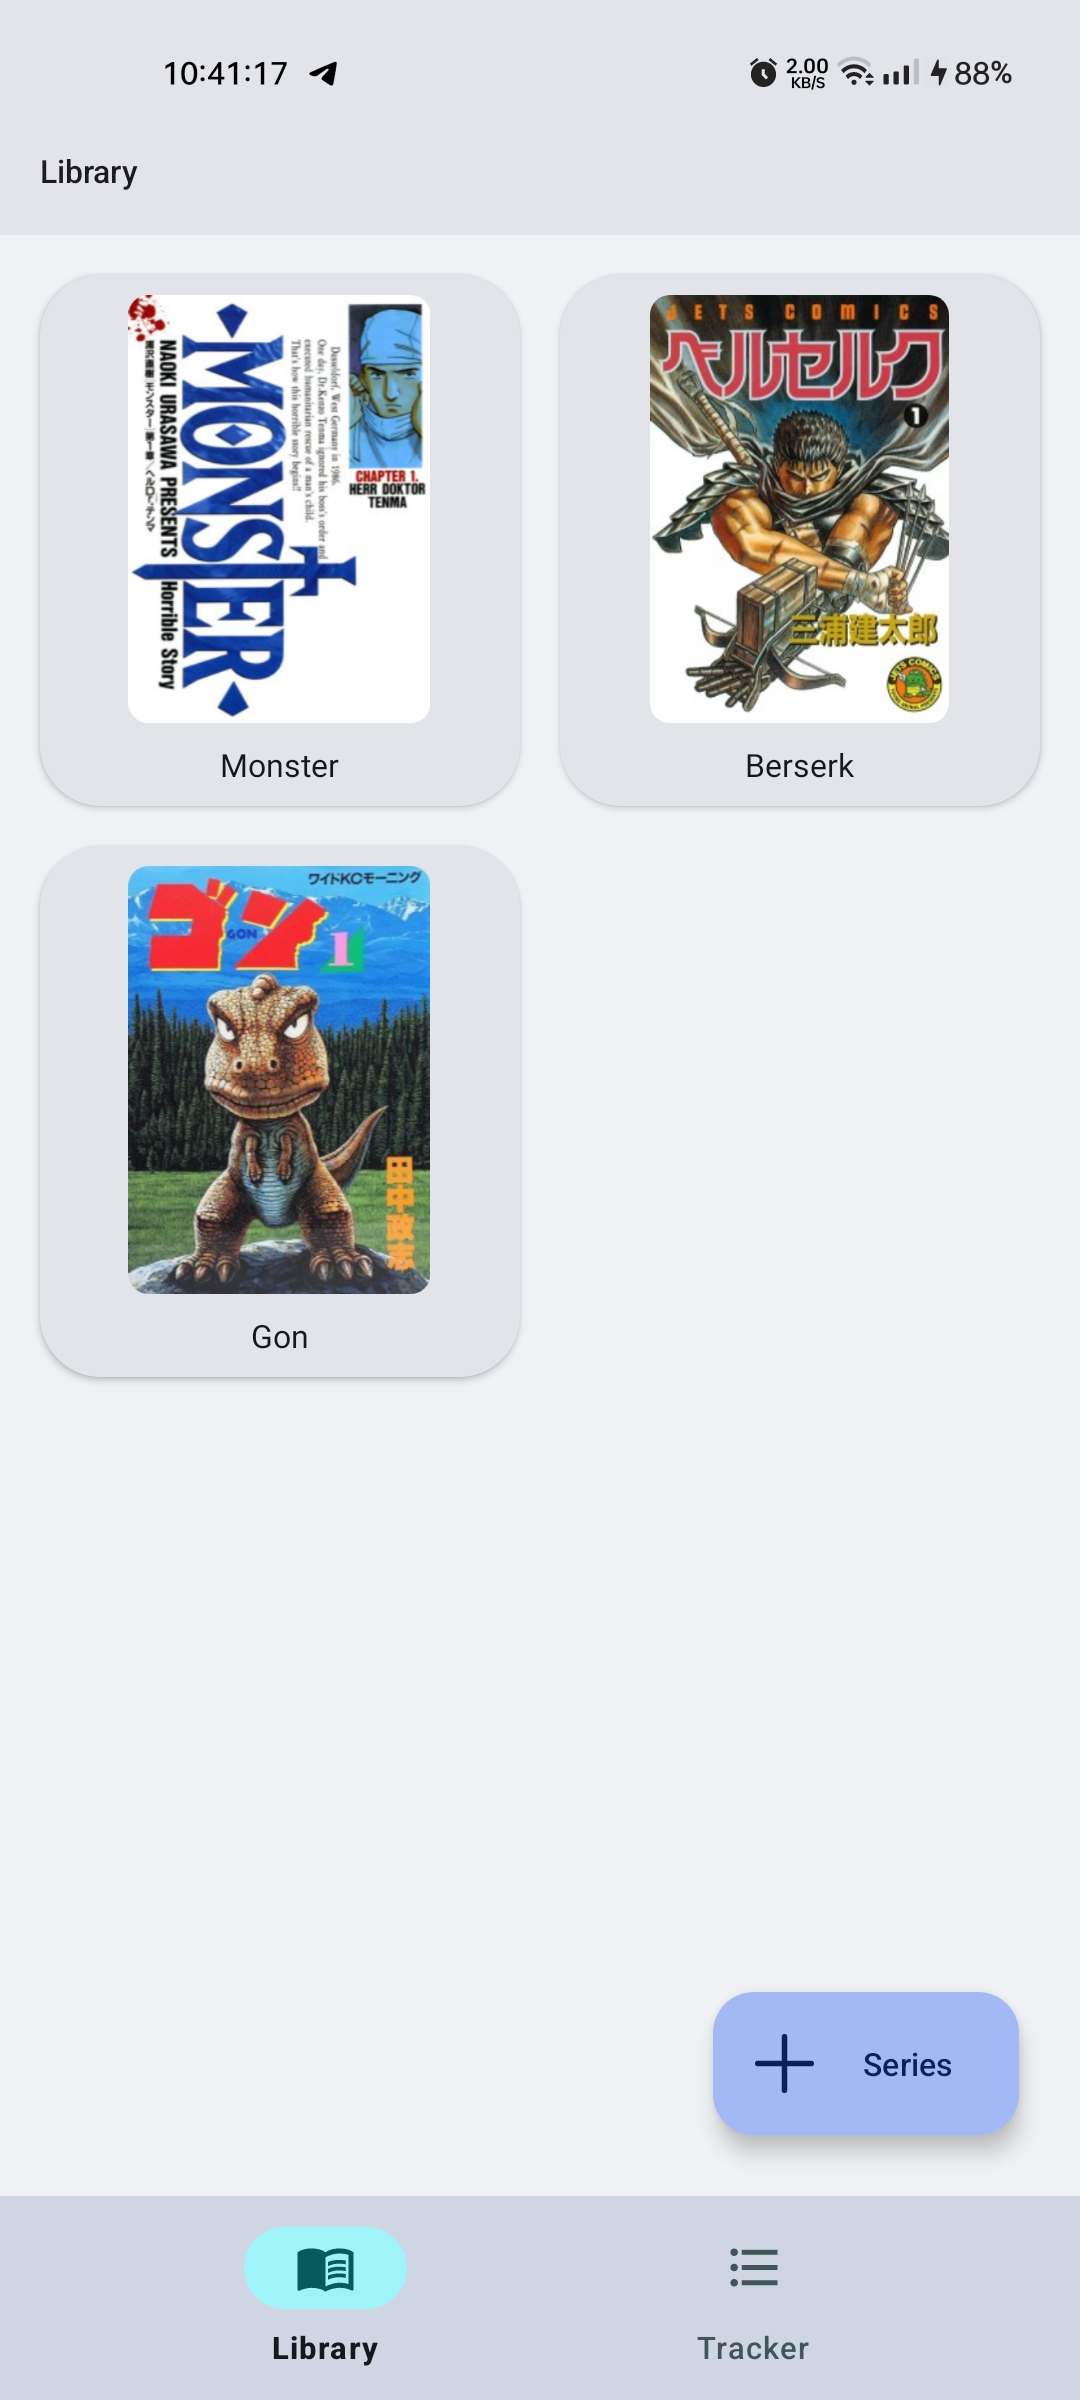
\includegraphics[scale=0.15]{library_redesign.jpg}
\end{center}

La home page non ha subito molte variazini.\\
Abbiamo però rimosso il menù ad hamburger in favore di una barra di stato nel alto inferiore dello schermo, e il pulsante di aggiunta di una serie specifica meglio cosa l'utente andrà ad aggiungere.

\subsection{Chapter list}\label{sec:ch_list_redesign}

\begin{center}
   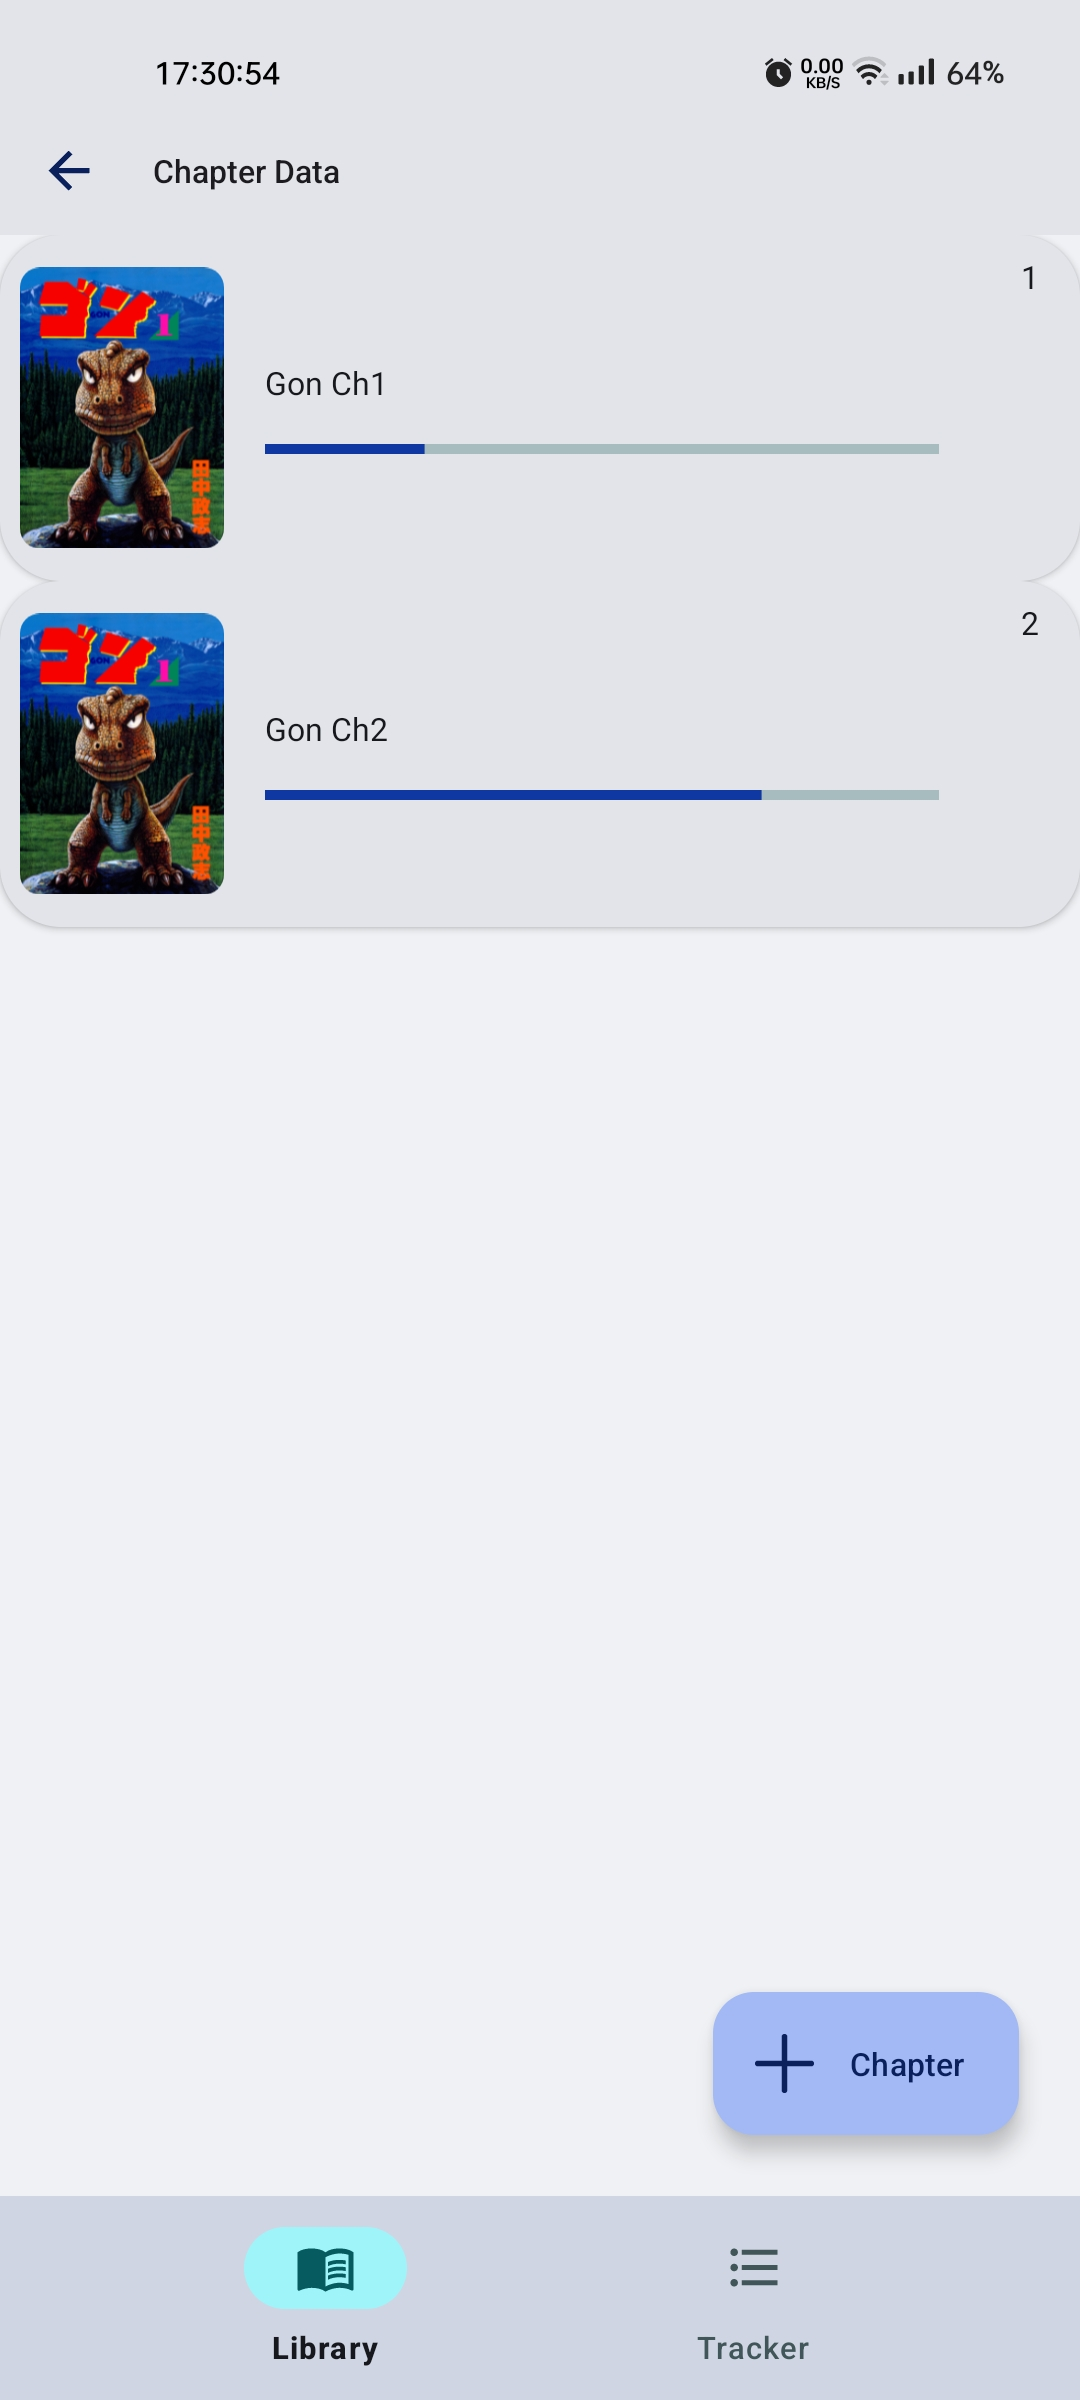
\includegraphics[scale=0.15]{chapter_list_redesign.jpg}
\end{center}

Ora la UI presenta delle isole più grandi per ogni capitolo di un'opera.\\
Le isole contengono tutte le informazioni, sulla base delle quali, l'utente potrebbe cercare un capitolo specifico, immagine di copertina nome e numero.\\
Nella parte inferiore delle isole c'è una barra di progressione che sta ad indicare la precentuale di lettura.\\
Come presente anche nella \hyperref[sec:home_redesign]{home page} è presente un bottone per l'aggiunta di una nuova risorsa, in questo caso di un capitolo.

\subsection{Add chapter}

\begin{center}
   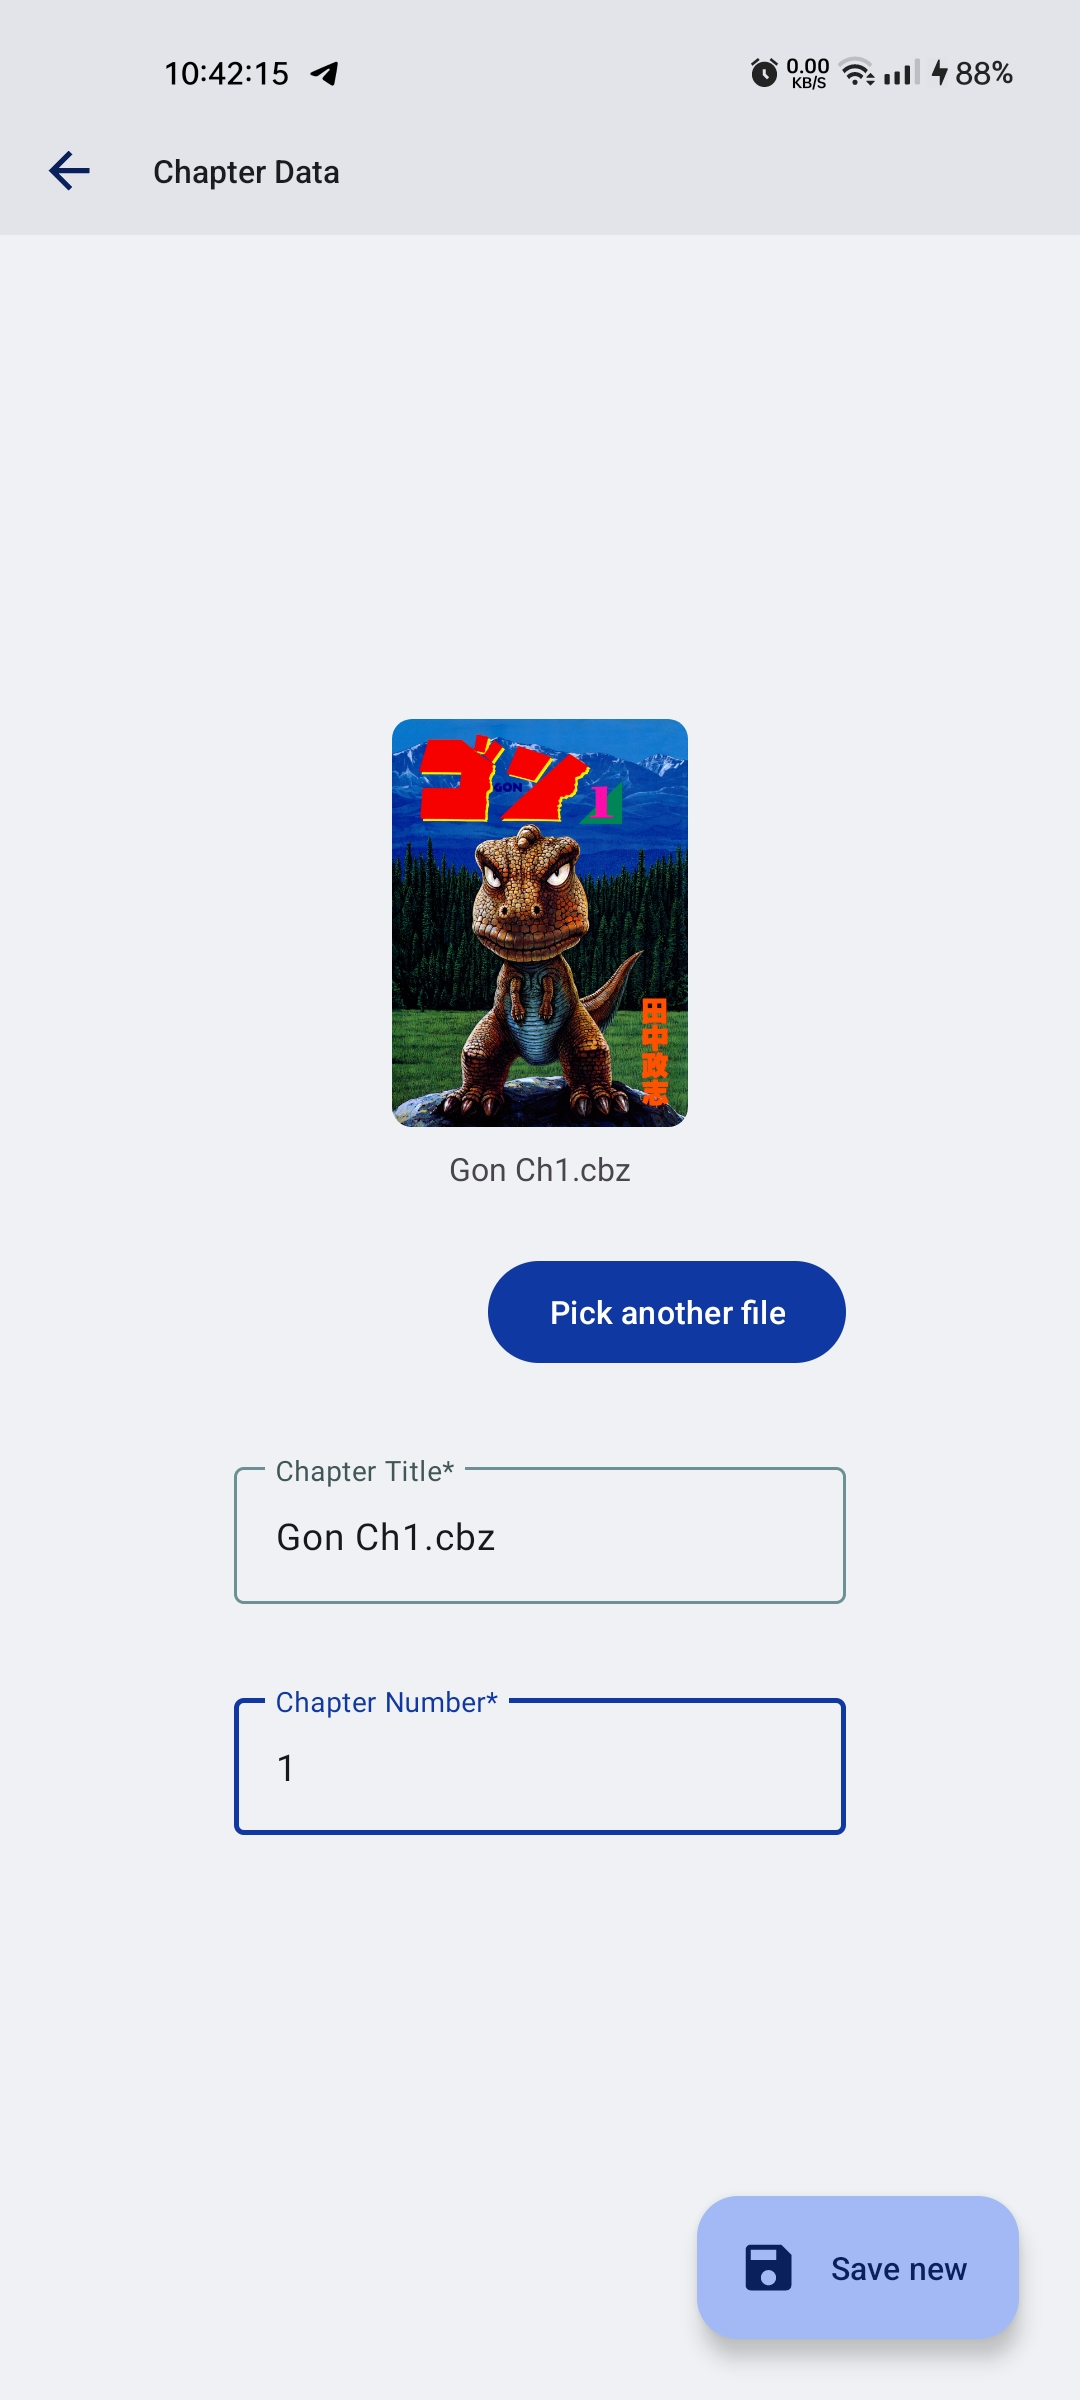
\includegraphics[scale=0.15]{add_chapter_redesign.jpg}
\end{center}

Dalla \hyperref[sec:ch_list_redesign]{lista dei capitoli}, premendo il pulsante di aggiunta, si verrà portati a questo form.\\
Verranno chieste all'utente solo le informazioni fondamentali come il file, il titolo da dare e il numero del capitolo.\\
All'utente prima della conferma apparirà un dialog indicante che le risorse non verranno portate nello spazio privato dell'applicazione, quindi se i file dovessero essere spostai non sarebbero più accessibili.

\subsection{Add series}\label{sec:add_series_redesign}

\begin{center}
   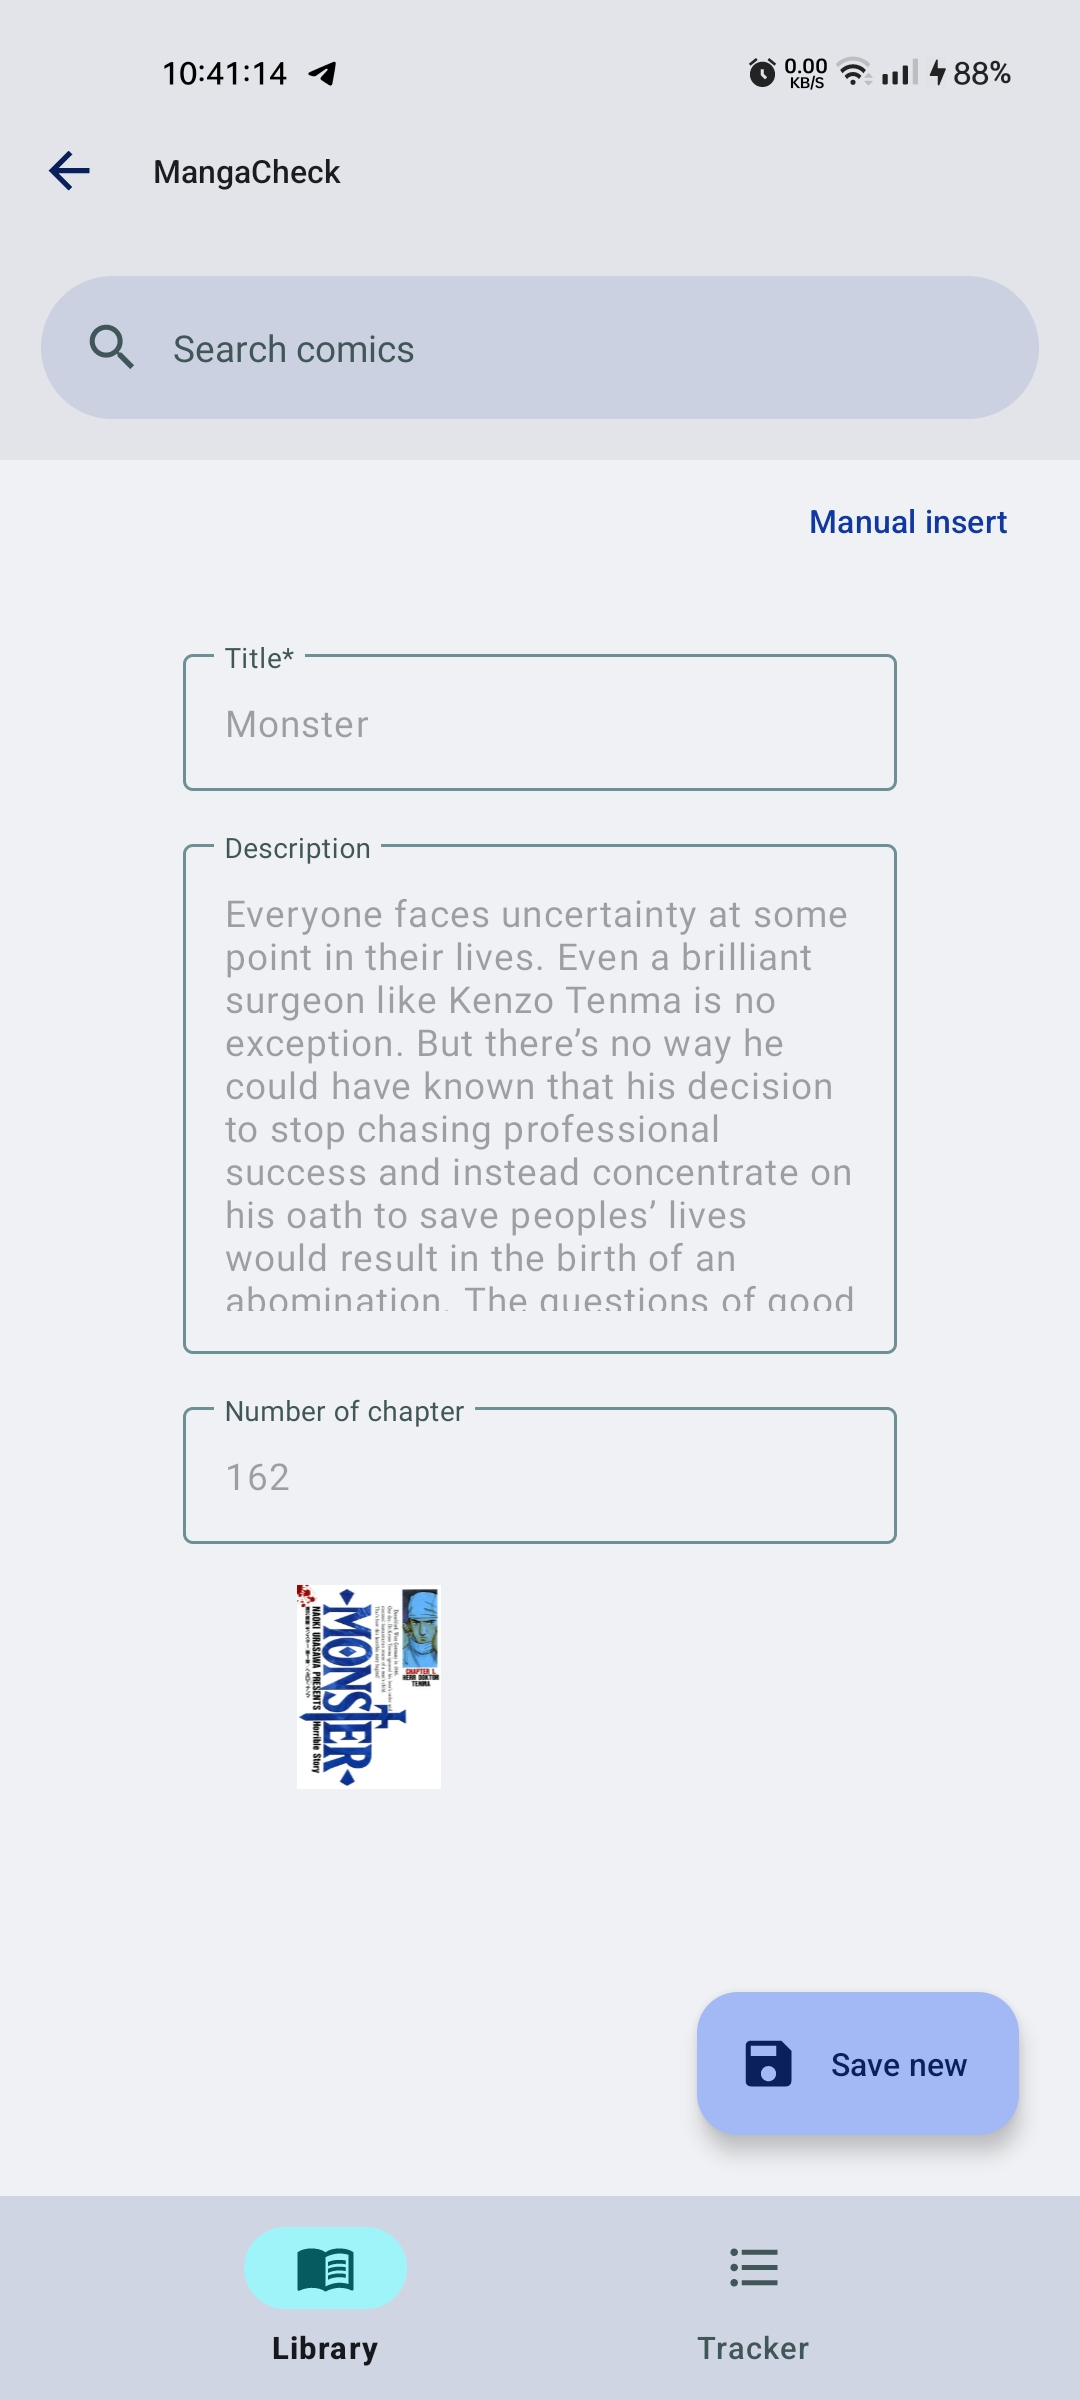
\includegraphics[scale=0.15]{add_series_redesign.jpg}
\end{center}

Abbiamo optato per una semplice barra di ricerca dalla quale visualizzare tutti i risultati inerenti alla stringa cercata.\\
Dopo aver premuto sul risultato cercato si aprirà un form per la conferma dei dati, i dati saranno presi dalle API di Anilist ma sarà comunque possibile per l'utente modificare i dati premendo nella voce in alto a destra.

\subsection{Tracker}

\begin{center}
   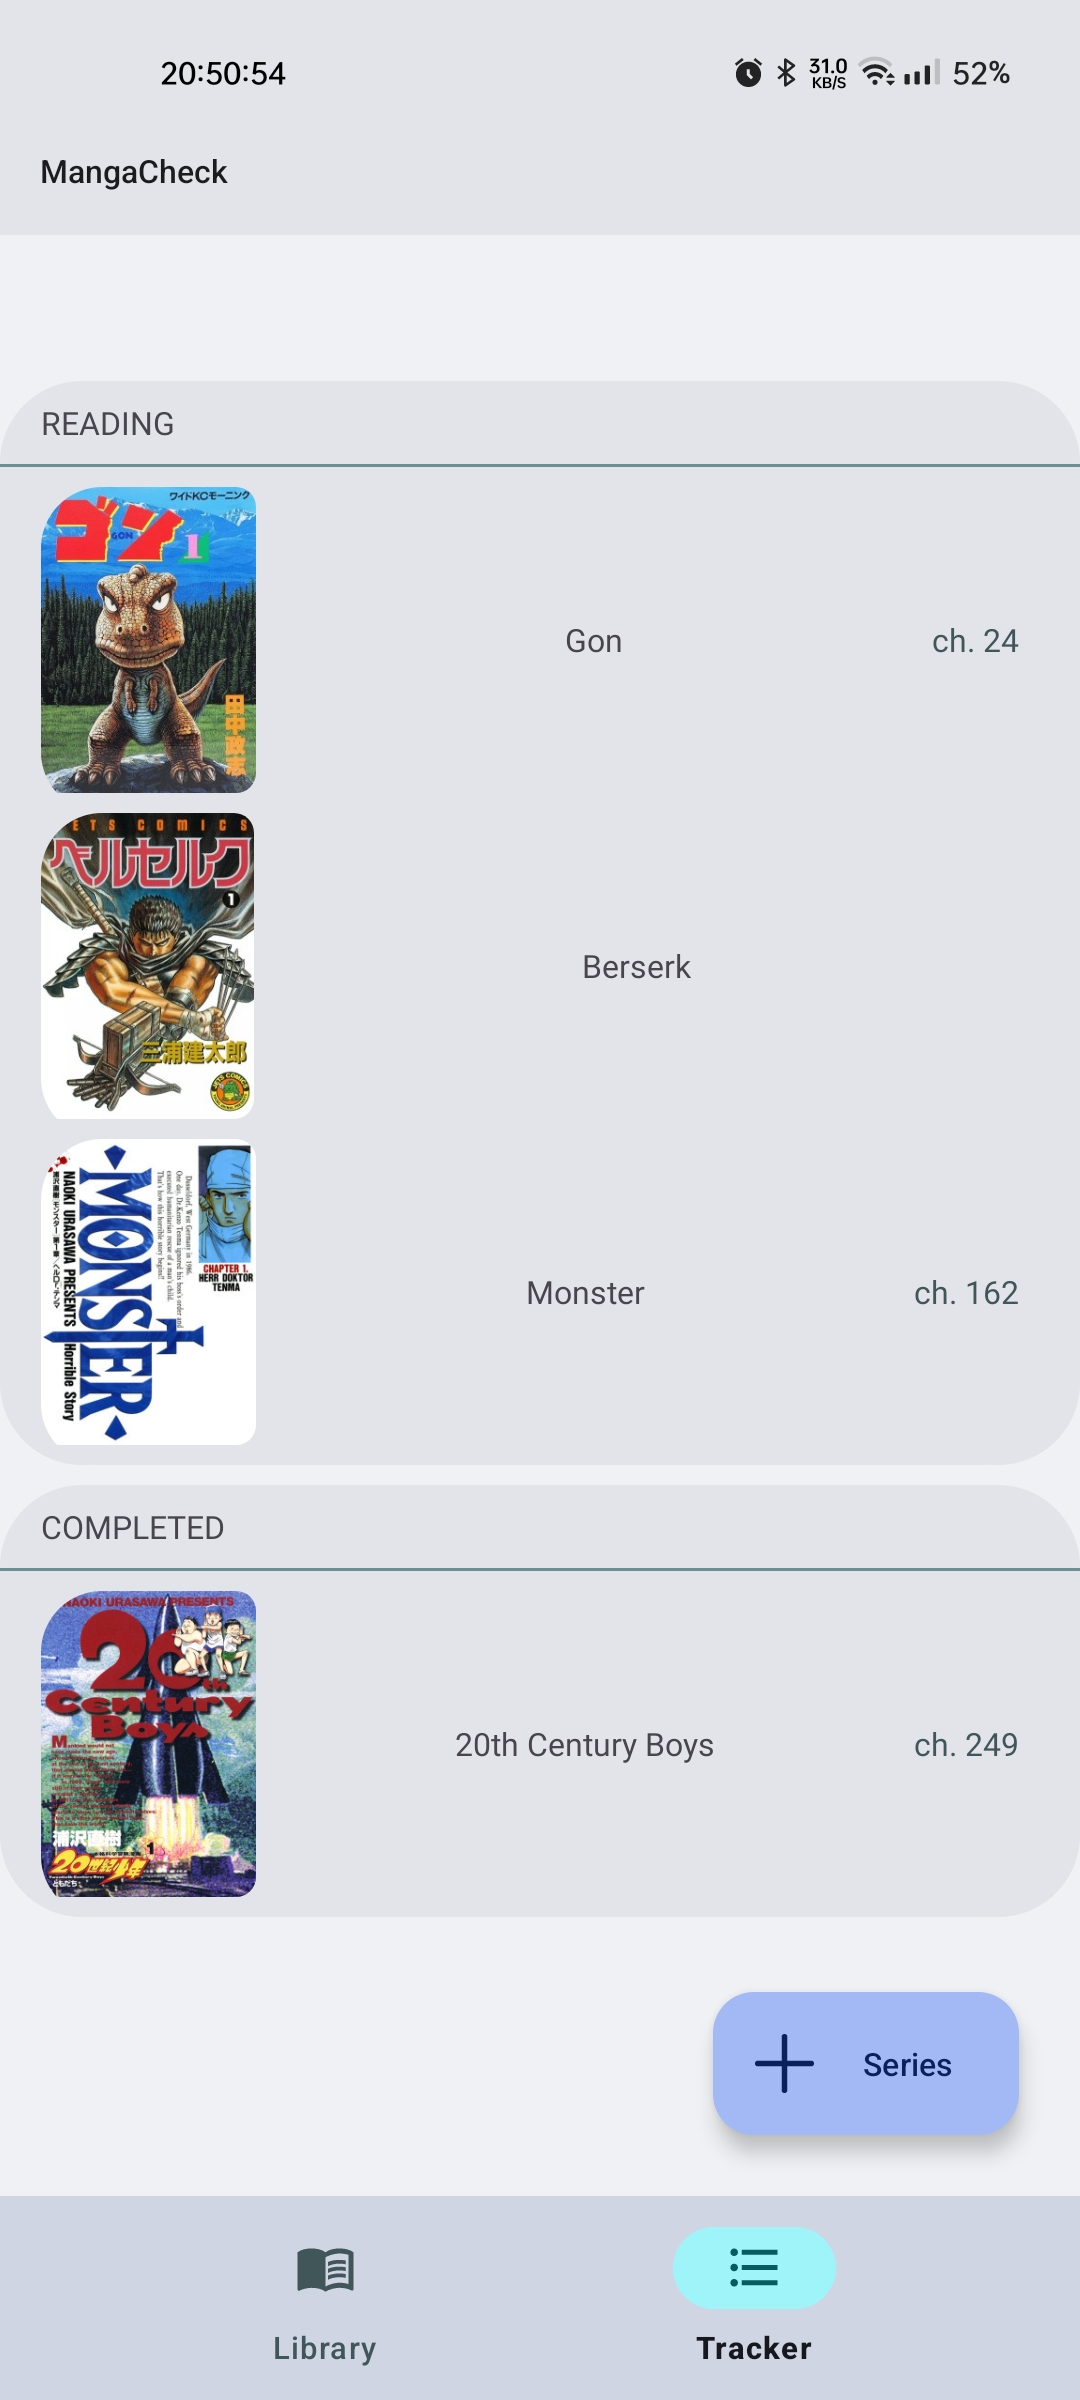
\includegraphics[scale=0.15]{tracker_redesign.jpg}
\end{center}

 Rispetto alla precedente \hyperref[sec:reading_list]{reading list} abbiamo aggiunto un'icona per esplicitare al meglio l'azione di modifica.\\
 Abbiamo mantenuto un bottone di aggiunta che riporta ad un form analogo a quello del \hyperref[sec:add_series_redesign]{add series}.\\
 Le series che vengono aggiunte alla \hyperref[sec:home_redesign]{libreria} vengono automaticamente aggiunte a questa sezione con lo stato di \texttt{READING}.\\
 Inoltre le voci presenti nella sezione \texttt{READING} sono clickabili e riportano all'ultimo capitolo aperto di quella serie, se non è presnte tale capitolo si viene riportati alla lista dei capitoli di tale opera.\\
 In caso di modifica verrà aperto un dialog tramite il quale l'utente potrà modificare lo stato di lettura di un'opera.

\subsection{Reader}

%\begin{center}
%   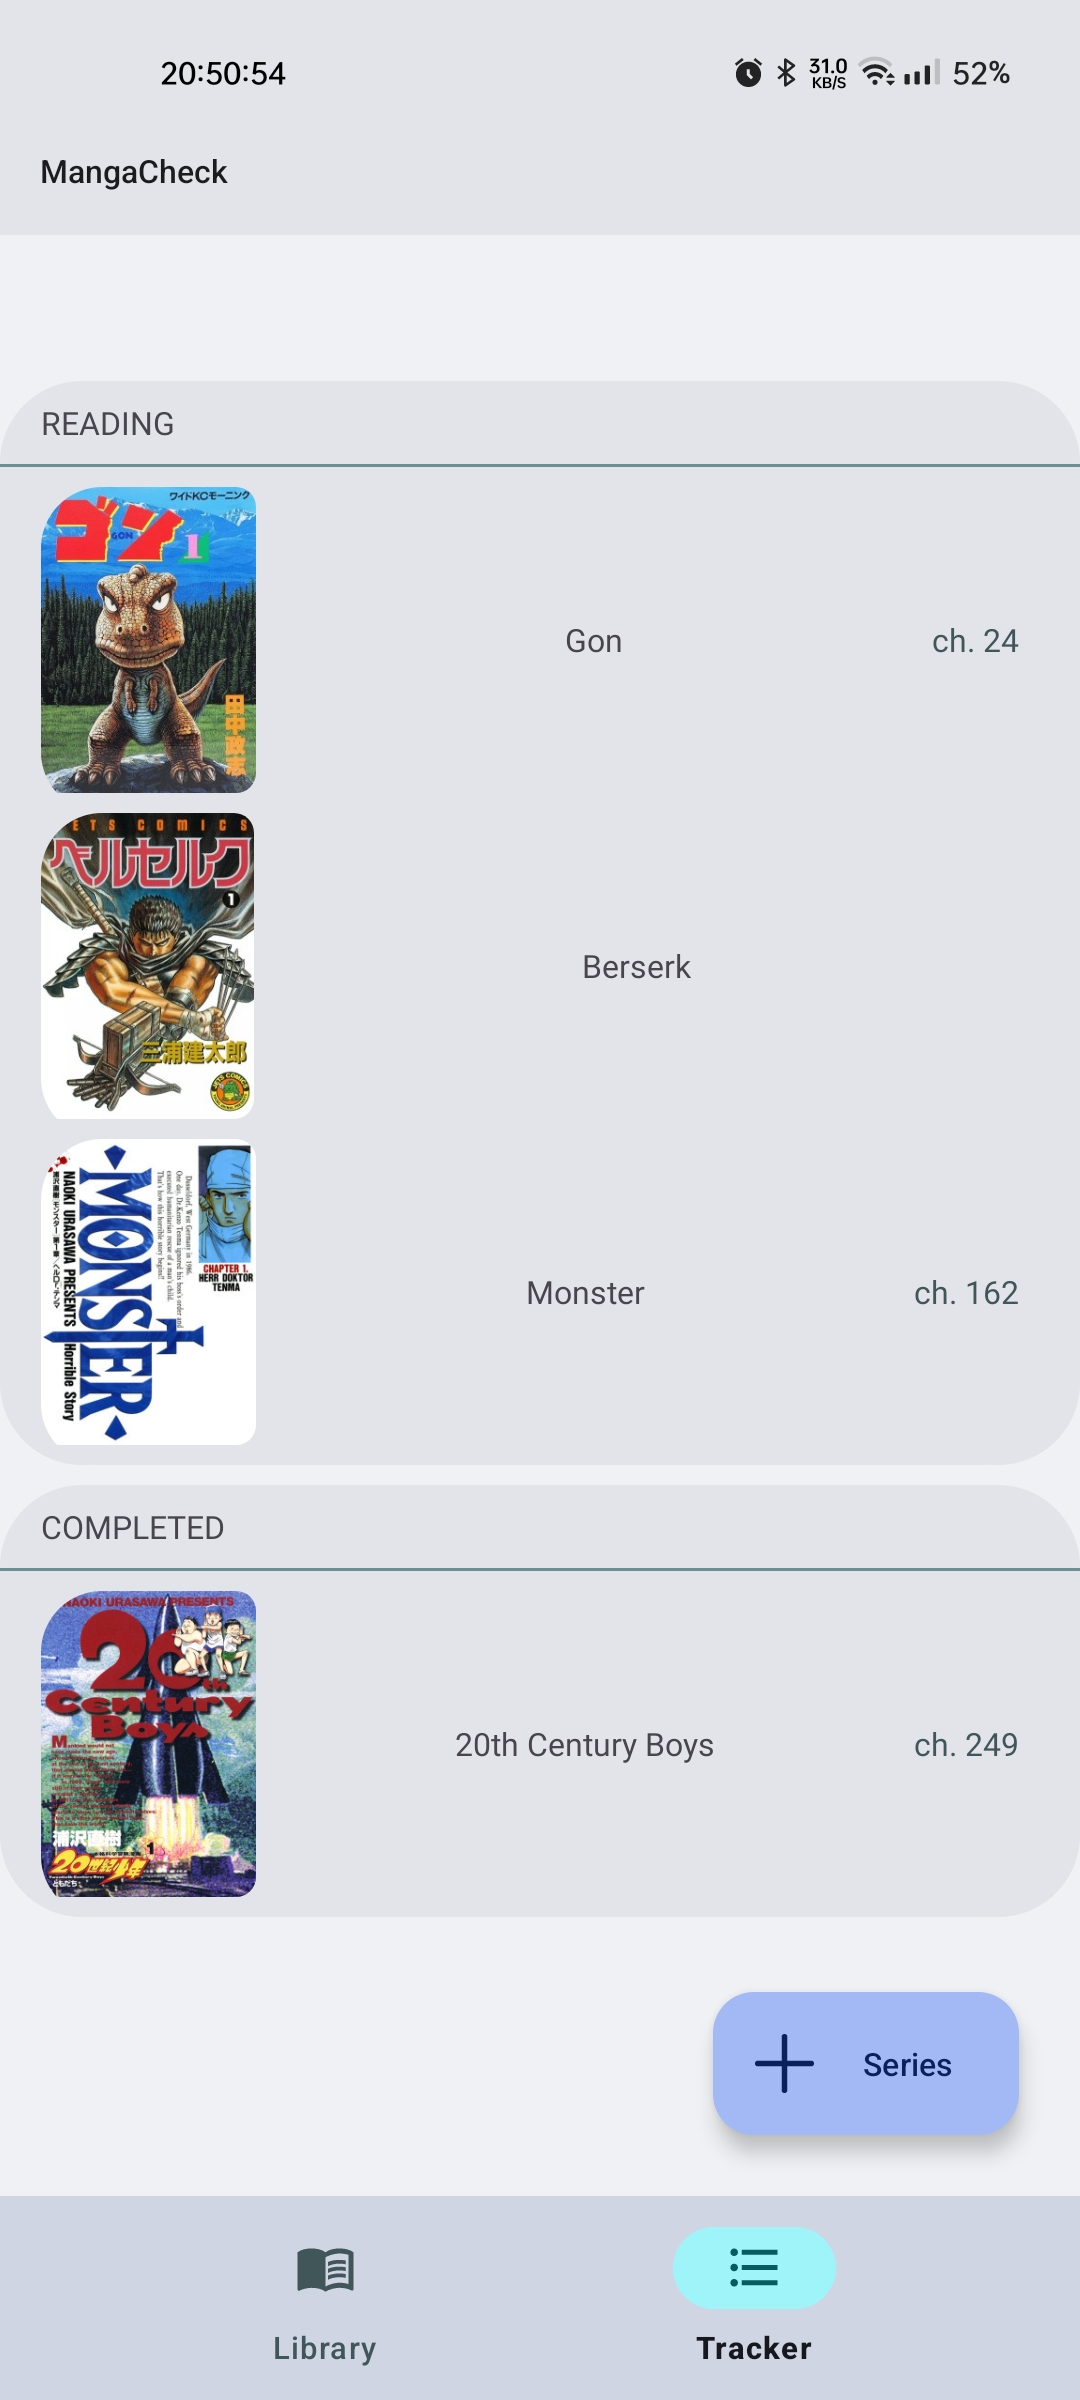
\includegraphics[scale=0.15]{tracker_redesign.jpg}
%\end{center}

Premendo su un capitolo l'utente verrà portato al reader, l'utente si potrà muovere tra le pagine con degli swipe a sinistra e destra.\\
Il Reader è stato implementato in modo tale che riprenda dall'ultima pagina che l'utente ha visualizzato.
Premendo sull'immagine appariranno una top bar e una bottom bar, nella bottom bar l'utente potrà trascinare il dito per scorrere velocemente tra le pagine.

\end{document}
